\newpage
\section{Lösungskonzept}
\subsection[Designkonzept]{Designkonzept}
Das Design des Admin-UIs wurde von einem seperaten Designerteam erstellt, welches nah mit dem Kunden zusammengearbeitet hat.

Die Mockups orientieren sich an den Anforderungen \hyperref[Tab:A4]{A4}, \hyperref[Tab:A5]{A5}, \hyperref[Tab:A6]{A6} und \hyperref[Tab:A7]{A7}. Sie fügen jedoch noch andere Elemente hinzu, um für ein gutes \acs{ux} zu sorgen. Dazu gehören:
\begin{itemize}
    \item Die Unterteilung der Eingabefelder mit der dazu passenden Überschrift.
    \item Platzhalter in den Eingabefeldern, um besser zu erkennen, was in die Felder eingetragen werden muss.
\end{itemize}

Anhand der Kundenanforderungen und den \acs{ux}-Anforderungen hat wurden von dem Designteam einige Mockups für das Admin-UI erstellt, welche dem Entwicklerteam als Leitbild dienen soll. \\\\
\textit{Notiz: Um die Anonymität des Kunden zu wahren, wurden einige Stellen der Mockups geschwärzt.}

\subsubsection[short]{Mockups für das Admin-UIs}
\begin{figure}[H]
    \centering
    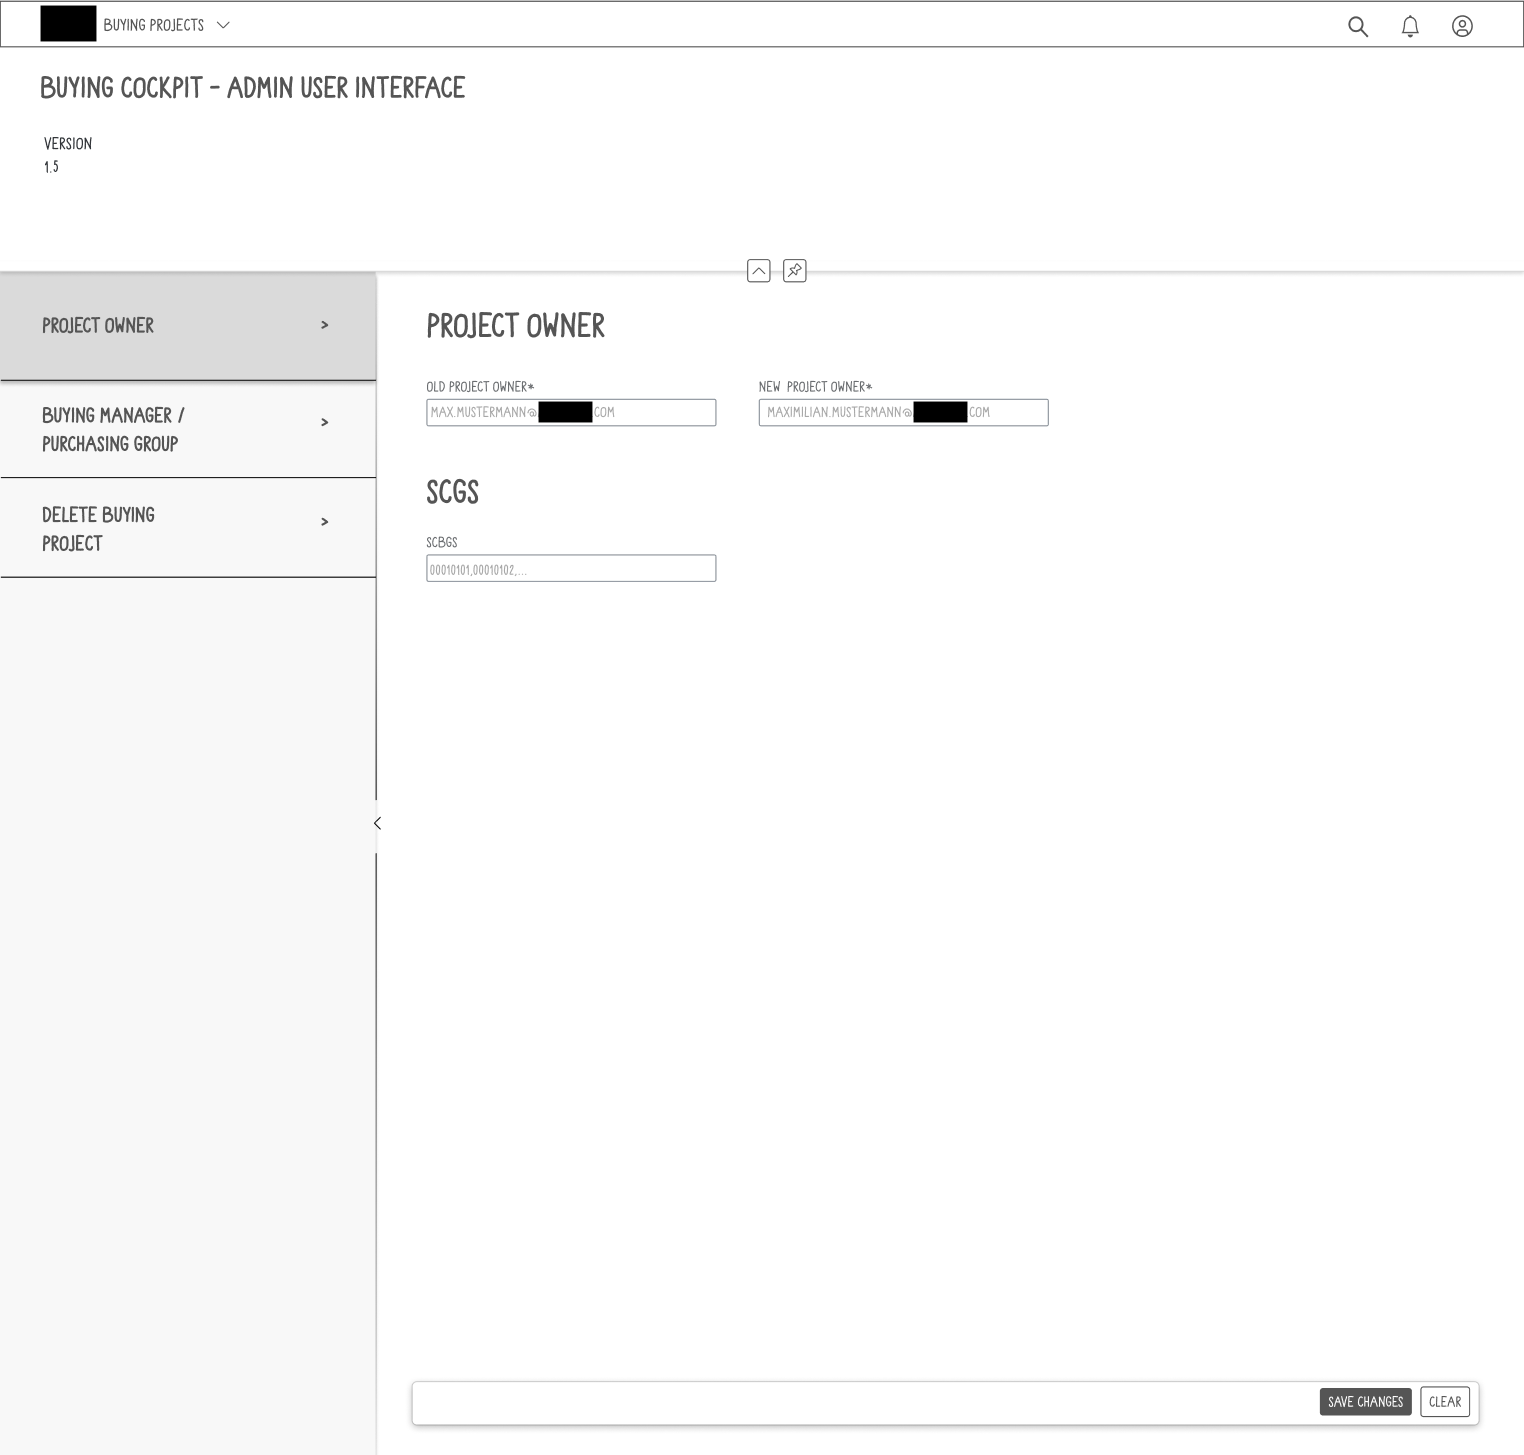
\includegraphics[width=\linewidth]{Images/Mockup_PO_anonym.png}
    \caption[Mockup: Admin-UI Projekowner Seite]{Mockup: Admin-UI Projekowner Seite}
\end{figure}

\begin{figure}[H]
    \centering
    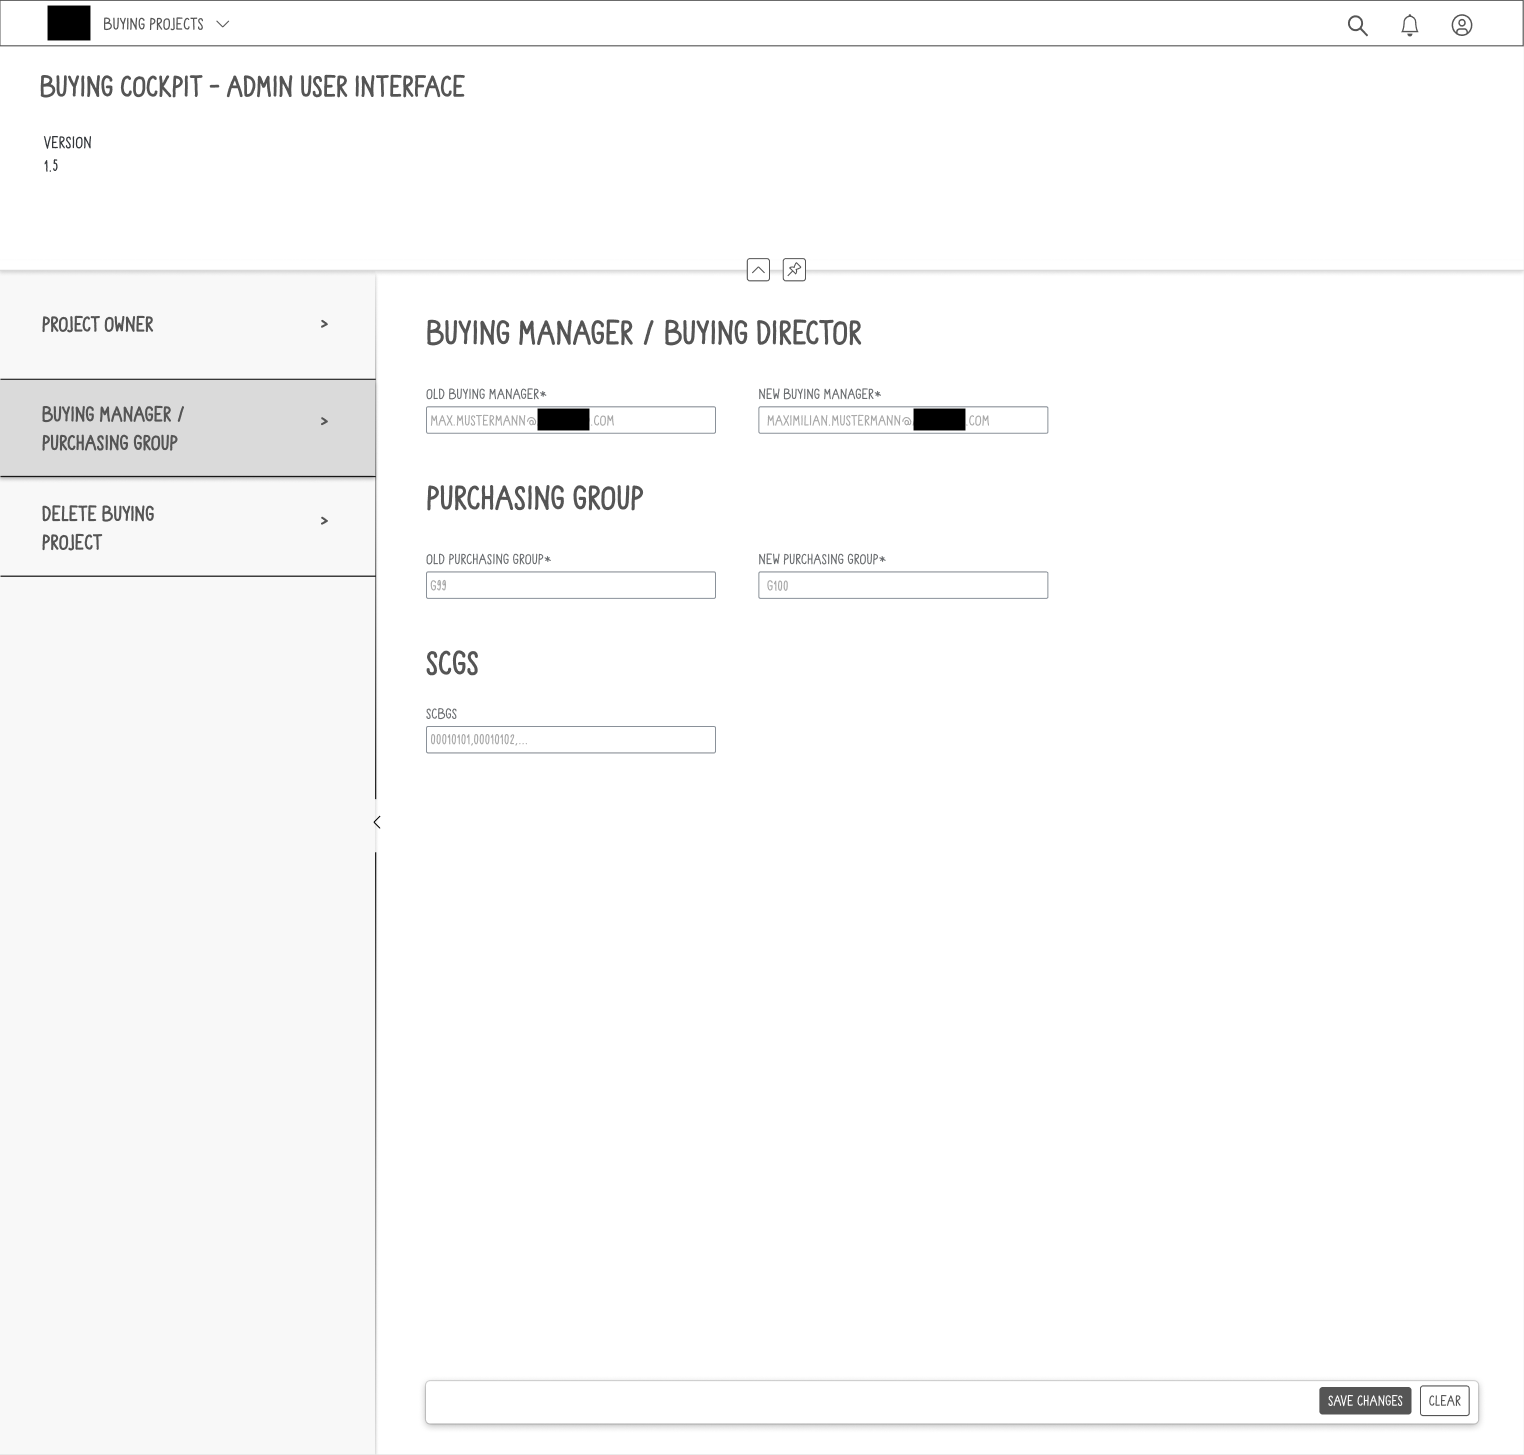
\includegraphics[width=\linewidth]{Images/Mockup_PM_anonym.png}
    \caption[Mockup: Admin-UI Projektmanager und Käufergruppe Seite]{Mockup: Admin-UI Projektmanager und Käufergruppe Seite}
\end{figure}

\begin{figure}[H]
    \centering
    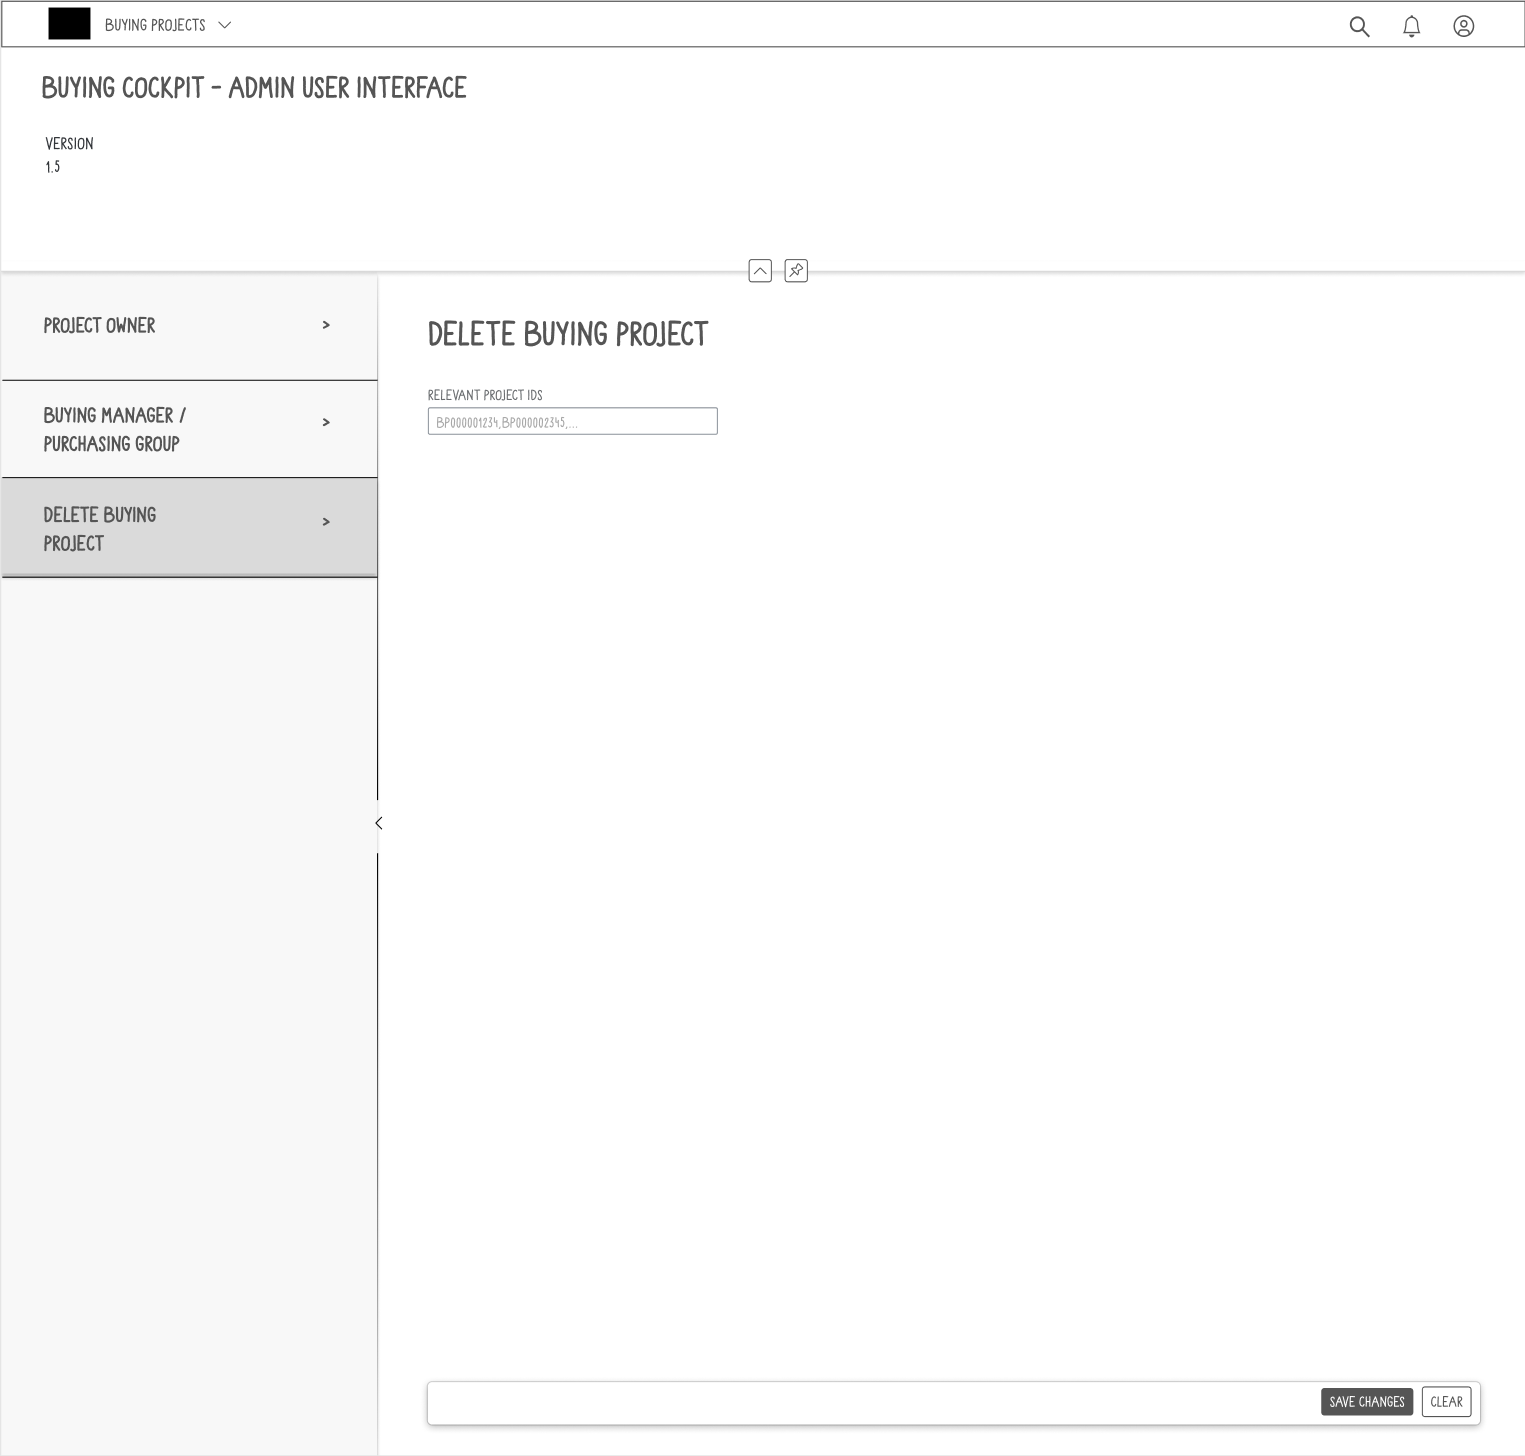
\includegraphics[width=\linewidth]{Images/Mockup_DEL_anonym.png}
    \caption[Mockup: Admin-UI Löschungs-Seite]{Mockup: Admin-UI Löschungs-Seite}
\end{figure}

\begin{figure}[H]
    \centering
    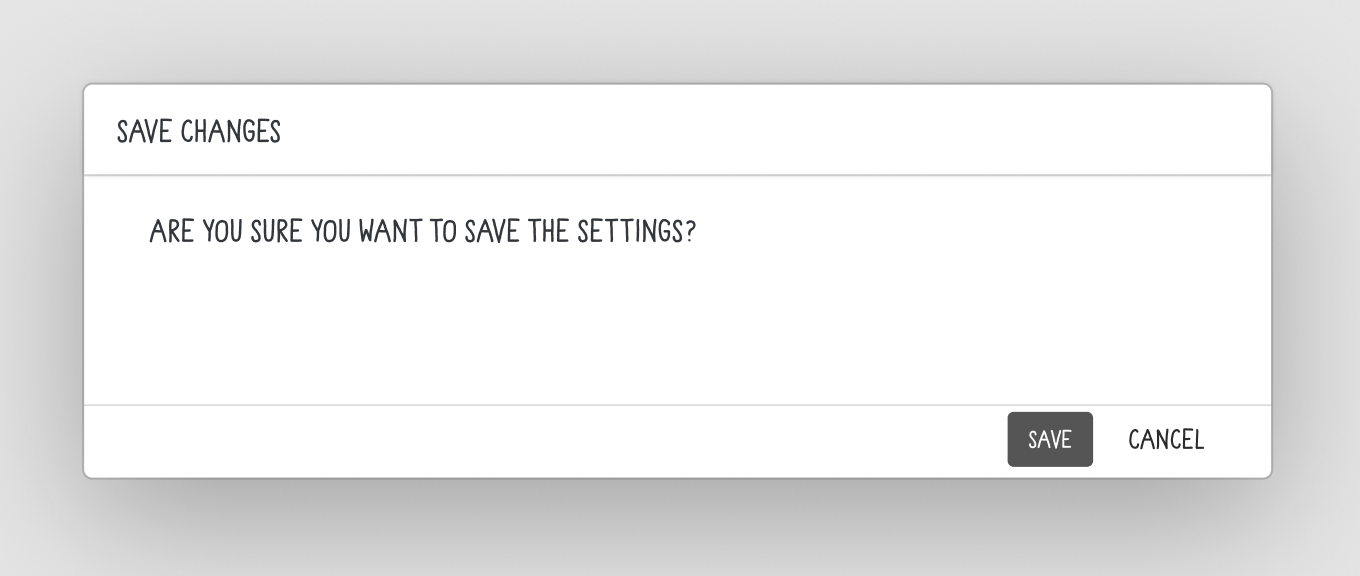
\includegraphics[width=\linewidth]{Images/Mockup_PopUp.png}
    \caption[Mockup: Admin-UI Pop-Up]{Mockup: Admin-UI Pop-Up}
\end{figure}

\subsection[Software-Design]{Software-Design}